\documentclass{article}


\usepackage{amsmath}
\usepackage{graphicx}
\usepackage{float}
\usepackage{polski}
\usepackage{subcaption}
\usepackage[margin=1.25in]{geometry}
\usepackage{minted}



\usepackage{caption}

\begin{document}
\begin{titlepage}
    \begin{center}
 
        
 
 
        \vspace{0.8cm}
		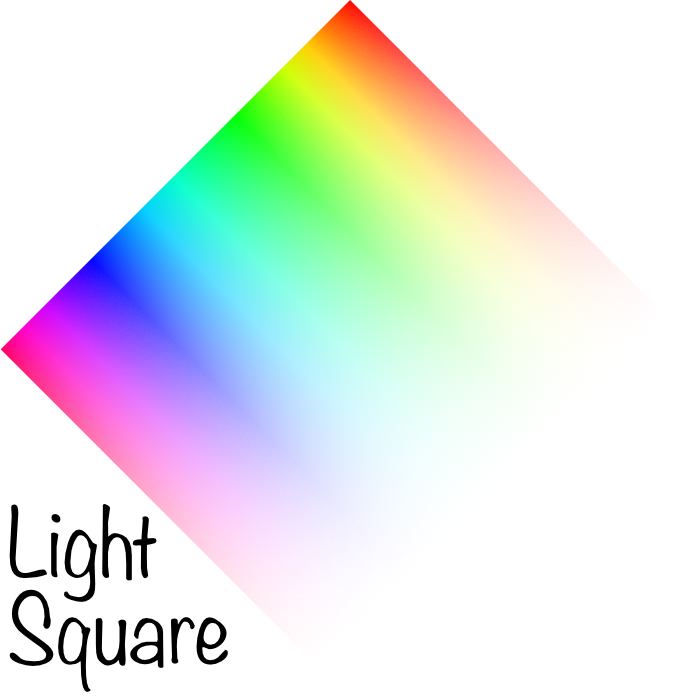
\includegraphics[width=\textwidth]{LightText2.png} 
 		\vfill
        \Large
        Karolina Romanowska 304120\\
        Michał Matak 304071\\
        Systemy Komputerowe w Sterowaniu i Pomiarach\\
        Informatyka\\
        Wydział Elektroniki i Technik Informacyjnych\\
        Politechnika Warszawska\\
 
    \end{center}
\end{titlepage}
\pagenumbering{gobble}
\pagenumbering{arabic}
\section{Wprowadzenie}
Celem projektu jest stworzenie szybko reagującego systemu przetwarzającego 4 gesty, dzięki któremu możliwe będzie sterowanie barwą oraz jasnością kwadratu znajdującego się na stronie serwera.
\section{Opis systemu}
\subsection{Opis środowiska}
Obraz systemu Linuks zostanie przygotowany przy pomocy Buildroota. Wykorzystana zostanie platforma wirtualna, dostarczona przez emulator QEMU, która będzie emulować komputer jednopłytkowy 64-bitowy o procesorze ARM z kamerą. Serwer będzie uruchomiony na maszynie gospodarza - komputerze z systemem operacyjnym Windows 10. 
\subsection{Działanie systemu z punktu widzenia użytkownika}
Działanie programu zostanie zainicjowane poprzez włączenie serwera, który to wyśle początkowe połączenie do płytki z informacją o rozpoczęciu korzystania z oprogramowania. Użytkownik wykonując odpowiedni gest przed kamerą podłączoną do komputera jednopłytkowego (klienta) chce zmienić kolor lub jasność światła w pokoju. Komputer jednopłytkowy rozpoznaje gest i wysyła dane o nim do serwera poprzez WiFi. Serwer odpowiednio modyfikuje parametry światła. W tym przypadku,w realizacji na maszynie wirtualnej, kamerą urządzenia będzie kamera laptopa, a jasność i kolor światła będą reprezentowane poprzez graficzny interfejs użytkownika. Planowane są 4 gesty:
\begin{table}[H]
\begin{tabular}{|l|l|}
\hline
ruch ręki w górę  & zwiększenie jasności kwadratu  \\ \hline
ruch ręki w dół   & zmniejszenie jasności kwadratu \\ \hline
ruch ręki w prawo & zmiana barwy na zimniejszą     \\ \hline
ruch ręki w lewo  & zmiana barwy na cieplejszą     \\ \hline
\end{tabular}
\centering
\end{table}
\subsection{Opis wymagań}
Od systemu wymagamy aby po wykonaniu gestu zmiana światła nastąpiła w czasie mniejszym niż jednej sekundy, nawet gdy klient znajduje się pod dużym obciążeniem.
\subsection{Schemat systemu}
\begin{figure}[H]
  \centering  
  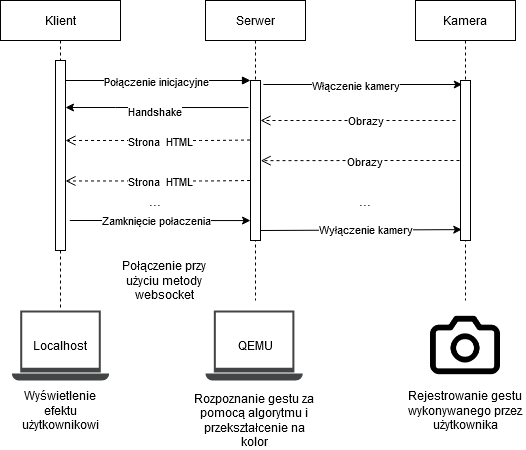
\includegraphics[width=0.8\linewidth]{sequence.png}
  \caption{Schemat systemu}
\end{figure}   
\subsection{Opis poszczególnych elementów systemu}
\section{Koncepcja rozwiązania}
\subsection{Stworzenie obrazu systemu}
Obraz jądra systemu zostanie stworzony za pomocą buildroota. Jako początkowa konfiguracja wybrana będzie qemu\_aarch64\_virt\_defconfig. W sekcji Toolchain należy wybrać External toolchain. W sekcji Filesystem initial RAM filesystem. Kompilacja dokona się po użyciu komendy make.
\subsection{Obsługa kamery}
Do obsługi kamery zostaną ściągnięte pakiety FFmpeg, libv4l oraz v4l-utils tools, ffmpeg zostanie załadowany poprzez wywołanie odpowiedniej opcji w Target packeges  Audio and video applications natomiast w pozostałych przypadkach libraries hardware handling.
\subsection{Rozpoznawanie gestu}
Wykorzystane technologie: Python i OpenCV
Zdecydowaliśmy się na rozpoznawanie 4 gestów dynamicznych. Chcemy użyć metody przetwarzania obrazu, rozpoznając ruch na podstawie kilku wybranych klatek. Użyjemy zaimplementowanych w bibliotece algorytmów OpenCV (niżej krótko opisanych)  i wybierzemy najszybszy i dający najlepszą dokładność.
\begin{table}[H]
\begin{tabular}{|l|l|l|l|}
\hline
Nazwa             & opis & zalety & wady \\ \hline
Meanshift         &      &        &      \\ \hline
Camshift          &      &        &      \\ \hline
Template matching &      &        &      \\ \hline
Przepływ optyczny &      &        &      \\ \hline

\end{tabular}
\centering
\end{table}
Następnie gest zostanie zinterpretowany i przyporządkowany do odpowiedniego numeru gestu. Ostatecznie odpowiednio wpłynie na wyświetlany kolor.
\subsection{Architektura klient serwer}
Wykorzystane technologie: Python, JavaScript, FastAPI, WebSockets, HTML, CSS, Uvicorn
Do implementacji architektury klient serwer wykorzystano technologię zapewniającą dwukierunkowy kanał komunikacji przy pomocy jednego połączenia TCP. Protokół ten zapewnia większą szybkość przesyłania danych w Internecie, dzięki czemu jest dobrym rozwiązaniem dla systemów czasu rzeczywistego. Jego działanie można przedstawić w paru prostych krokach: klient wysyła żądanie HTTP do serwera, połączenie zostaje nawiązane (tzw. handshake). Następnie dane swobodnie przepływają między klientem a serwerem. Połączenie inicjalizowane jest przez klienta - rozpoczyna się wtedy również przechwytywanie obrazu z kamery, następnie gdy połączenie zostanie nawiązane, przetworzone dane na kolor trafiają szybko do klienta. Gdy ten uzna że zakończył korzystać z usługi - zamyka połączenia a kamera przestaje przechwytywać obraz. 
\subsection{Połączenie internetowe}
W systemie wykorzystamy dwustronne połączenie lokalne do przesyłania strony HTML’owej dla klienta z odpowiedniego koloru obrazem. Planujemy do tego wykorzystać bezprzewodową sieć komputerową. 
Konfiguracja w Buildroocie
 W sekcji “Networking support” należy wybrać Wireless - obsługę sieci bezprzewodowej. Następnie w sekcji “Wireless” należy zaznaczyć cfg80211 - wireless configuration API  i Generic IEEE 802.11 Networking Stack (max80211). Cfg80211 to interfejs API do konfiguracji dla urządzeń, który łączy przestrzeń użytkownika i sterowniki, IEEE 802.11 jest standardem opisującym sieć Wi-Fi. Kolejnym krokiem jest wybranie w sekcji “Device Drivers/Network device support” opcji Wireless LAN. Dalej należy zaznaczyć sterowniki dla bezprzewodowych kart sieciowych z interfejsem USB - Realtek 8187 i 8187B USB support. Ostatnią rzeczą jest dodanie potrzebnych do późniejszej konfiguracji sieci pakietów - iw - oprogramowanie umożliwiające kontrolę i zarządzanie kartami bezprzewodowymi i wpa\_supplicant - do obsługi standardu szyfrowania stosowanego w sieciach Wi-Fi. Następnie należy zbudować system i połączyć się z wybraną siecią.
\subsection{Stworzenie wersji wykonywalnej i umieszczenie na QEMU}
\subsection{Działanie pod dużym obciążeniem}
Aby zapewnić jak największa szybkość działania planujemy zwiększyć priorytety procesów odpowiedzialnych za rozpoznawanie obrazów, aby scheduler przydzielał im pierwszeństwo w obsłudze przez jądro. Jeśli to rozwiązanie nie wystarczy do spełnienia wymagań, to rozważymy także stworzenie obszaru pamięci dzielonej, w którym producentem będzie program rozpoznający gesty, a konsumentem program wysyłający je oraz usunięcie niepotrzebnych elementów z systemu.
\section{Testowanie}
\subsection{Stworzenie obrazu systemu}
Informacje o tym czy udało się stworzyć żądany obraz, poda nam komenda ‘make’ wykonana w katalogu buildroot’a. Sprawdzenia czy obraz posiada dane/ umożliwia dane funkcje sprawdzimy podczas testowania tych funkcji.
\subsection{Obsługa kamery}
To czy kamera jest poprawnie podłączona i obsługiwana przez qemu, a także czy załączyliśmy do buildroota wszystkie wymagane w tym celu załączniki zamierzamy sprawdzić wykonując prostą komendę ją obsługującą z konsoli:
        ffmpeg -f video4linux2 -r 30 -s 640x480 -i /dev/video0 out.avi
\subsection{Rozpoznawanie gestu}
W ramach pierwszych testów nagrane zostanie kilka filmików, które algorytmy będą musiał poprawnie przetworzyć i rozpoznać. Następnie zostaną porównane i wybrany najlepszy z nich zgodnie z kryteriami zamieszczonymi w opisie.  Później przeprowadzone zostaną testy z użyciem kamery w czasie rzeczywistym na wybranym już algorytmie. Ostatnim testem będzie sprawdzenie poprawności przesłania danych o geście do serwera. Ciekawym eksperymentem będzie również sprawdzenie jak zachowa się algorytm przy poruszaniu obrazem rejestrowanym przez kamerę, gdzie nie ma człowieka wykonującego gest.
\subsection{Architektura klient serwer}
Testowane odbędzie się przy pomocy biblioteki pytest, gdzie sprawdzane będą kody odpowiedzi serwera na żądanie klienta oraz poprawność wyświetlanego koloru.
\subsection{Połączenie internetowe}
Pierwszym testem będzie diagnozowanie połączenia sieciowego przy pomocy polecenia Ping. Następnie przy pomocy stworzonej architektury klient serwer sprawdzone zostanie połączenie, szybkość wysyłanych danych, oraz przypadek w którym sieć zawiedzie i połączenie zostanie utracone.
\subsection{Działanie pod dużym obciążeniem}
Aby sprawdzić czy nasz projekt spełnia to wymaganie planujemy odpalić na qemu program, który będzie wykonywał daną operacje (np. atoi(“a”)) odpowiednio dużą liczbę razy (np. 50 000 000).
\section{Analiza literatury}
\end{document}